\documentclass[conference]{IEEEtran}

\usepackage{amsmath,amssymb,amsfonts,amsthm}
\usepackage{mathrsfs}
\usepackage{algorithm}
\usepackage{algpseudocode}
\usepackage{booktabs}
\usepackage{tabularx}
\usepackage{array}
\usepackage{makecell}
\usepackage{multirow}
\usepackage{url}
\usepackage{graphicx}
\usepackage{xcolor}
\usepackage{float}
\usepackage{placeins}

\setlength{\textfloatsep}{7pt plus 1pt minus 2pt}
\setlength{\floatsep}{7pt plus 1pt minus 2pt}
\setlength{\intextsep}{7pt plus 1pt minus 2pt}
\setlength{\dbltextfloatsep}{7pt plus 1pt minus 2pt}
\setlength{\dblfloatsep}{7pt plus 1pt minus 2pt}
\setlength{\abovecaptionskip}{3pt}
\setlength{\belowcaptionskip}{0pt}

\newtheorem{definition}{Definition}[section]
\newtheorem{assumption}{Assumption}[section]
\newtheorem{theorem}{Theorem}[section]
\newtheorem{corollary}{Corollary}[section]
\newtheorem{lemma}{Lemma}[section]

\newcommand{\eps}{\epsilon}
\newcommand{\ldp}{\mathrm{LDP}}
\newcommand{\pow}{\mathrm{PoW}}
\newcommand{\TEE}{\mathrm{TEE}}
\newcommand{\V}{\mathscr{V}}
\newcommand{\MSE}{\mathsf{MSE}}
\newcommand{\RMSE}{\mathsf{RMSE}}
\newcommand{\NoVerify}{\textsc{NoVerify}}
\newcommand{\DirectAttest}{\textsc{DirectAttest}}
\newcommand{\RejectMismatch}{\textsc{RejectMismatch}}
\newcommand{\TEEOnly}{\textsc{TEEOnly}}
\newcommand{\AuditSlash}{\textsc{AuditSlash}}
\newcommand{\StrongDeposit}{\textsc{StrongDeposit}}
\newcommand{\ReputationOnly}{\textsc{ReputationOnly}}
\newcommand{\TEEPOW}{\textsc{TEE-PoW}}
\newcommand{\Hybrid}{\textsc{SealedHybrid}}
\newcommand{\SealedClass}{\textsc{SealedClass}}

\title{Budget Integrity and Quality-Claim Verification for LDP Data Products}

\author{\IEEEauthorblockN{Yadi Wen, Ruijie Xing, Yaling Ren, Dan Yu, Rong Du, Yue Fu, Yongle Chen}
\IEEEauthorblockA{Shanxi Key Laboratory of Industrial Internet Security, Taiyuan University of Technology, China\\
Emails: \{2023005322, 2024002195, 2023006489\}@link.tyut.edu.cn, \{yudan, durong, fuyue, chenyongle\}@tyut.edu.cn}}

\begin{document}
\maketitle


\begin{abstract}
Data marketing platforms increasingly sell LDP data products such as audience counts, segment-reach estimates, conversion-rate sketches, and campaign-lift reports. We study a budget-integrity problem in these markets: a seller may advertise a high-utility privacy budget $\eps_c$ while the local randomizer that produced the report actually used a stricter budget $\eps_h<\eps_c$. The report remains formally private, but the product is noisier and should be priced lower. Output-only validation is unreliable because LDP specifies a distributional guarantee and usually does not identify which executable, SDK, browser module, operating-system service, or trusted component performed the perturbation.

The strongest design is direct attestation of the realized budget whenever exact $\eps_h$ may be disclosed. This paper addresses markets where exact-budget disclosure is restricted while coarse quality classes can be public. Such sealed-class contracts arise when exact budgets reveal a private price book, negotiated cohort terms, privacy-ledger state, anti-gaming thresholds, or cross-contract governance constraints. We introduce a budget-integrity certificate for LDP reports and instantiate it with a TEE-sealed local oracle. The oracle emits one LDP report, attests executable identity, freshness, and a public quality class, and keeps $\eps_h$ and random coins sealed. Attestation, reject-on-mismatch, audit/slashing, deposits, and reputation are the primary controls; proof-of-work is an optional residual cost signal for rate limiting or for markets where escrow is unavailable. The evaluation combines workload-aware valuation, exact-disclosure baselines, a Criteo-style marketing workload, real AWS Nitro Enclaves measurements, a 2.76M-report scaled Nitro run, incentive sweeps, robustness tests, and adaptive-attacker studies.
\end{abstract}

\begin{IEEEkeywords}
Data markets, data marketing, data valuation, budget integrity, quality-claim verification, local differential privacy, trusted execution environments, AWS Nitro Enclaves, audits, deposits, proof-of-work.
\end{IEEEkeywords}


\section{Introduction}

Data markets no longer sell only raw tables. A modern data-marketing platform often sells derived data products: noisy audience counts, cohort-level histograms, segment-reach estimates, campaign-lift measurements, conversion-rate sketches, and feature summaries exposed through dashboards or APIs. These products are database objects in the ICDE sense: they have schemas, workloads, freshness contracts, provenance, query plans, and service-level objectives. Their value depends on whether the released statistics are accurate enough for downstream decisions such as budget allocation, inventory forecasting, look-alike audience construction, and fraud monitoring.

Local differential privacy (LDP) is a natural privacy layer for these products. Each user randomizes their own record before any market, broker, or buyer observes it, which weakens the need to trust a central curator~\cite{duchi2013local,kasiviswanathan2011what,erlingsson2014rappor,Wang2017LDPFreq}. The formal LDP definition, however, abstracts away a systems detail that matters in a market. It says that a local randomizer $R_\eps$ maps an input $x$ to a randomized output $y$ with a bounded likelihood ratio, but it generally does not say which executable or module performed that perturbation. The report may have been produced by an approved SDK, a browser module, a JavaScript snippet, an operating-system telemetry service, a vendor binary, a secure element, or a TEE. A buyer therefore observes a perturbed report and a claimed privacy budget, but may not know whether the approved local randomization path was used.

This missing execution identity is the source of the oracle abstraction. The oracle is not a second privacy model and does not convert LDP into centralized DP. It is a minimal, local, attested execution boundary that answers a systems question left open by LDP: which trusted module ran the randomizer, under which sealed budget policy, and with which freshness counter? The oracle consumes one local record, produces one LDP report, and releases no raw data. Its output is a report plus market metadata that can be stored, priced, audited, and joined with other marketplace controls.

\textbf{Threat.} We study privacy-budget fraud. A seller markets a data product as if it were generated with budget $\eps_c$, but locally randomizes records with a stricter budget $\eps_h<\eps_c$. In common LDP families, smaller $\eps$ means more randomization, higher estimation error, and lower buyer utility. The seller can then charge for a high-utility product while delivering a lower-value one. The attack is not a privacy violation; it is a market-integrity and valuation failure. Because the output is still LDP under $\eps_h$, a verifier needs execution identity and budget-policy evidence rather than output-only tests.

\textbf{Model boundary.} The paper focuses on LDP data products whose value is tied to query answers such as counts, reach estimates, and conversion sketches. Centralized DP has a different trust boundary because a curator selects and runs the release mechanism. Training-oriented mechanisms produce different outputs and are not part of the evaluation. This boundary keeps the mechanism aligned with data marketing, query valuation, and local randomization.

\textbf{Approach.} We design a budget-integrity certificate for LDP reports and instantiate it with a TEE-sealed local oracle. A market first chooses a disclosure regime. If exact $\eps_h$ may be disclosed, \DirectAttest{} or \RejectMismatch{} is the appropriate gate. If contracts expose only a coarse quality class, the oracle attests code identity, policy version, freshness, report commitment, and the public class while keeping exact $\eps_h$ sealed. The remaining class-boundary premium is handled by residual controls configured by the market: audits and slashing, monetary deposits, reputation, admission deadlines, or optional PoW.

\begin{figure*}[t]
\centering
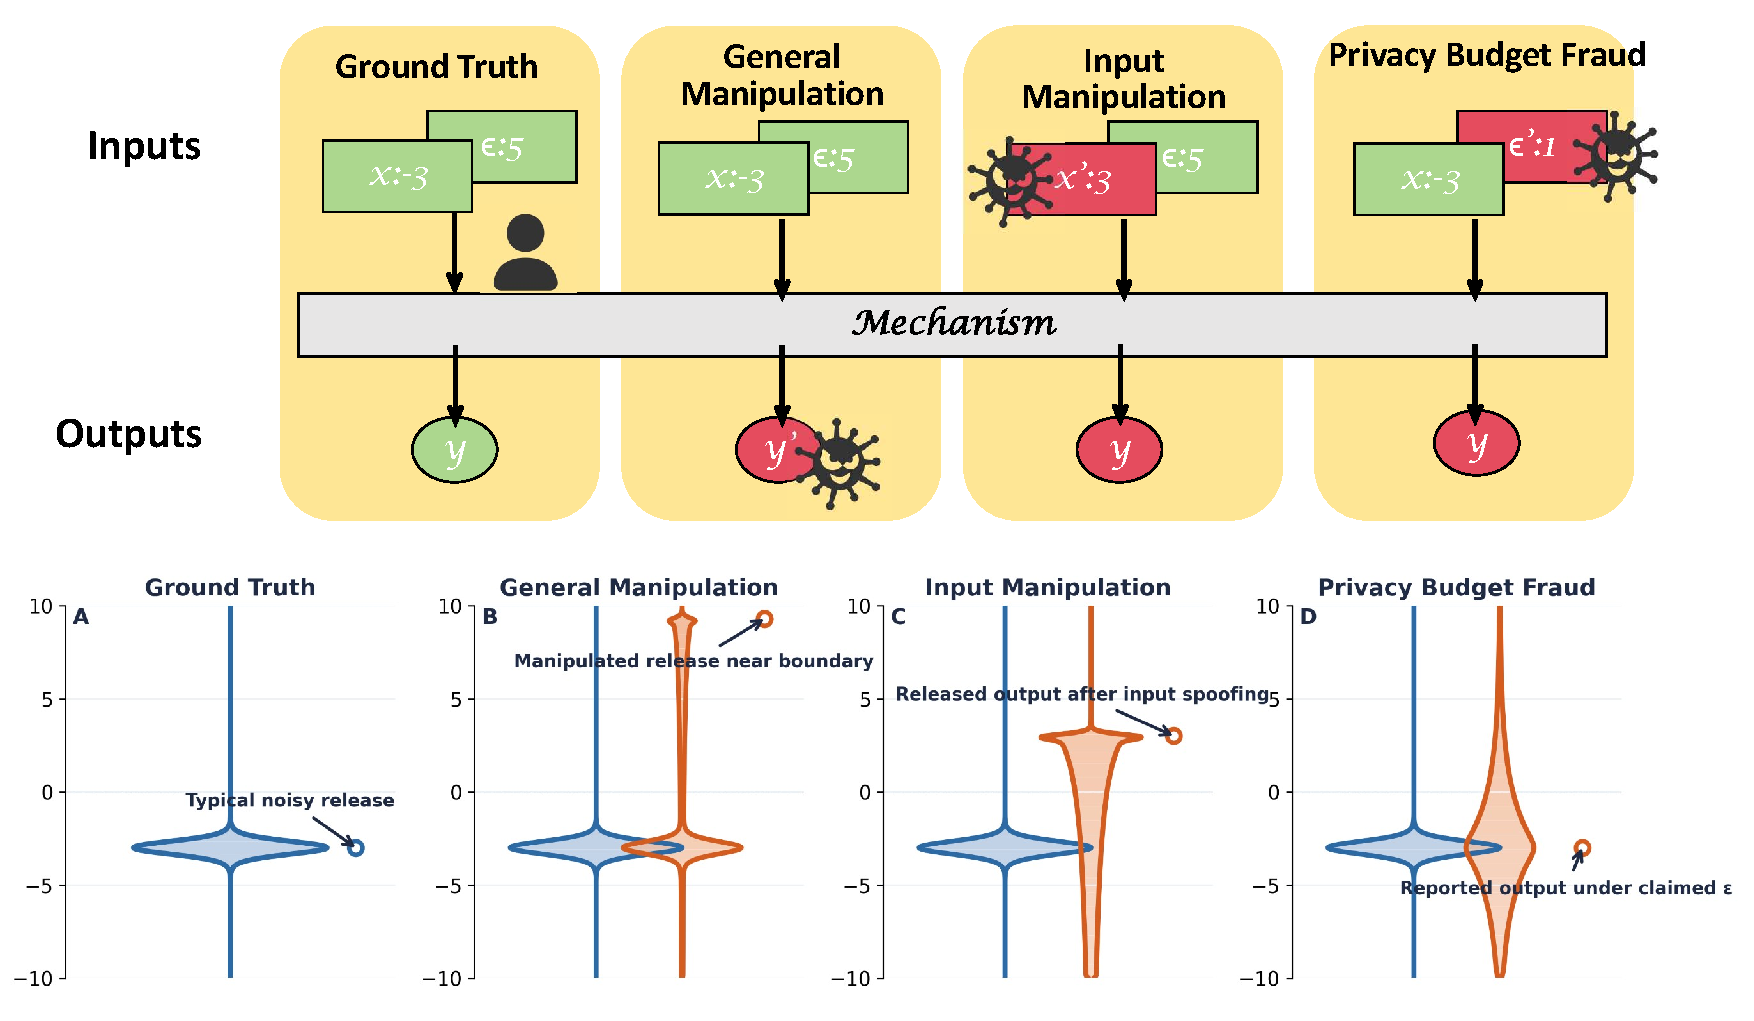
\includegraphics[width=0.86\textwidth]{figure1.pdf}
\caption{Privacy-budget fraud is a budget-claim attack distinct from output manipulation and input spoofing.}
\label{fig:fraud-taxonomy}
\end{figure*}

Fig.~\ref{fig:fraud-taxonomy} separates the attack from broader manipulation. Output manipulation changes the released value after the mechanism, while input manipulation spoofs the local record before randomization. Privacy-budget fraud instead uses the approved LDP family but runs it under a stricter hidden budget while marketing the product under the higher claimed budget. The output can remain plausible and private, which is why the certificate binds the report to the randomizer identity and budget policy rather than to a statistical after-the-fact test.

\textbf{Contributions.} First, we formulate LDP privacy-budget over-claims as a database-market integrity problem for queryable data products. Second, we define a budget-integrity certificate: a market metadata object that binds an LDP report to code identity, workload, public quality class, freshness, and the enforcement policy used for pricing. Third, we characterize disclosure regimes and treat \DirectAttest{} and \RejectMismatch{} as first-class exact-disclosure baselines. Fourth, we give commercial, contractual, and governance reasons for sealed-class markets in which exact $\eps_h$ is not public. Fifth, we analyze residual controls that compose audits, deposits, reputation, deadlines, and optional PoW, and evaluate them on valuation tasks, an advertising-style workload, AWS Nitro Enclaves measurements, and adaptive attacker simulations.


\section{Related Work}

\textbf{Data pricing and valuation.} Query-based data pricing studies how database systems assign prices to views, queries, and derived information products~\cite{koutris2012query,li2014pricing}. Later systems work studies arbitrage-free pricing and scalable query-pricing frameworks~\cite{deep2017design,qirana2017}. Privacy-aware valuation and private-data markets link utility, procurement, auctions, and prices to privacy guarantees~\cite{ghosh2011selling,chen2022privacy,chen2023privacy,lei2024privacy}. Algorithmic marketplace work emphasizes task-dependent value and matching~\cite{agarwal2019marketplace}. These works price information products or allocate data tasks; our question is whether the budget and quality class used to price an LDP product can be verified after the report is generated by an untrusted local host.

\textbf{Marketplace metadata and provenance.} Provenance research explains how database systems attach lineage and trust metadata to derived results~\cite{buneman2001provenance,green2007provenance}. A budget-integrity certificate plays a similar systems role for LDP markets. It is not itself a price, estimator, or privacy proof, but it gives the pricing and audit layers a queryable record of randomizer identity, workload, freshness, public quality class, and enforcement policy. This separates our contribution from estimator design and places it closer to metadata infrastructure for derived data products.

\textbf{Local differential privacy and verification.} LDP was formalized in the theoretical literature and has been deployed for telemetry and frequency estimation~\cite{duchi2013local,kasiviswanathan2011what,erlingsson2014rappor,Wang2017LDPFreq}. Prior work studies manipulation and poisoning in LDP reports~\cite{cheu2021manipulation,cao2021data,wu2021poisoning}; verifiable randomization makes the randomization step harder to manipulate~\cite{kato2021verifiable}. Privacy odometers and filters study adaptive privacy accounting~\cite{rogers2016odometers}. These techniques address the privacy distribution, adversarial reports, or accounting over multiple releases. We study a complementary market failure: a report may be correctly randomized and still be mispriced if the seller over-claims the realized budget or public quality class.

\textbf{Residual controls and market deterrence.} Signaling games explain how costly signals separate higher-quality from lower-quality sellers~\cite{spence1973job}. Deposits, audits, and reputation are common market controls. PoW provides a tunable computational cost, but its latency, energy use, and fairness depend on hardware and strategic behavior~\cite{back2002hashcash,nakamoto2008bitcoin,kroll2013economics,eyal2014majority}. We therefore treat PoW as an optional residual signal rather than as the main mechanism. In low-latency data markets, exact disclosure, rejection, deposits, audits, and reputation are the primary controls.

\textbf{Trusted execution.} Trusted execution environments provide attested code identity and sealed state~\cite{costan2016intel}. Systems such as VC3, Opaque, and EnclaveDB show how TEEs can support trusted analytics over untrusted infrastructure~\cite{schuster2015vc3,zheng2017opaque,priebe2018enclavedb}. AWS Nitro Enclaves provide isolated EC2 execution environments with cryptographic attestation and platform measurements~\cite{awsnitro,awsattest}. We use TEEs for a narrower data-market primitive: certifying the LDP perturbation path and public quality class while leaving exact budgets sealed when the contract requires it.

\section{LDP Data-Market Model}
\label{sec:model}

\subsection{Data Products and Workloads}

A data-marketing product is a tuple
\[
\mathcal{P}=(\mathcal{X},R_\eps,\mathcal{Y},W,n,\mathsf{SLA}),
\]
where $\mathcal{X}$ is the local record domain, $R_\eps:\mathcal{X}\rightarrow\mathcal{Y}$ is an LDP randomizer family, $W$ is a buyer workload, $n$ is the expected number of reports, and $\mathsf{SLA}$ captures latency, freshness, and availability. Typical workloads include frequency estimation for audience categories, top-$k$ segment discovery, reach estimation, campaign-lift estimation, and conversion-rate reporting.

\begin{definition}[$\epsilon$-local differential privacy]
\label{def:ldp}
A local randomizer $R_\eps:\mathcal{X}\to\mathcal{Y}$ satisfies $\eps$-LDP if, for all $x,x'\in\mathcal{X}$ and all measurable $S\subseteq\mathcal{Y}$,
\[
\Pr[R_\eps(x)\in S]\le e^\eps\Pr[R_\eps(x')\in S].
\]
The guarantee is local because randomization occurs before the report leaves the user's boundary.
\end{definition}

For a fixed workload $W$, let $\mathcal{I}_W(\eps)$ denote the per-report information available to the workload-specific estimator. For randomized response and related frequency estimators, $\mathcal{I}_W(\eps)$ is increasing in $\eps$ because reports become less randomized. Let $\MSE_W(n,\eps)$ be the mean-squared estimation error for $n$ accepted reports. We use the estimator-level relationship
\[
\MSE_W(n,\eps)\ge \frac{1}{n\mathcal{I}_W(\eps)}
\]
as a valuation guide; equality is not required for our mechanism.

\begin{definition}[Workload-aware valuation]
\label{def:valuation}
The buyer value for product $\mathcal{P}$ under realized budget $\eps$ is
\[
\V_W(n,\eps)=B_W-L_W\big(\MSE_W(n,\eps)\big)-\Lambda_W(\mathsf{SLA}),
\]
where $B_W$ is the business value of a perfectly accurate product, $L_W$ is an increasing loss in estimation error, and $\Lambda_W$ is an SLA penalty. We assume $\V_W$ is nondecreasing in $\eps$ for fixed $W,n,$ and SLA.
\end{definition}


\subsection{Budget-Integrity Certificates}
\label{subsec:certificate}

The market-visible object produced by the verifier is a budget-integrity certificate. It is a small metadata record attached to an LDP report or to an aggregate batch. The certificate does not reveal the raw record and, in sealed-class mode, does not reveal exact $\eps_h$. It binds the report to the approved randomizer, the workload, the public quality signal, and the control used by the pricing rule.

\begin{table}[t]
\caption{Budget-integrity certificate schema used by the market verifier.}
\label{tab:cert-schema}
\centering
\scriptsize
\begin{tabularx}{\columnwidth}{p{0.27\columnwidth}X}
\toprule
Field & Role in the data-market pipeline \\
\midrule
Report commitment & binds $y$, salt, session id, workload id, and seller id \\
Randomizer identity & records code measurement, algorithm family, and policy version \\
Quality signal & exact $\eps_h$ under direct attestation, or a coarse class under sealed-class contracts \\
Freshness state & carries verifier nonce and monotone counter to reject replay \\
Residual control & records audit/deposit/reputation action or optional PoW bucket \\
Pricing hook & links the accepted certificate to posted price, auction score, or SLA payment \\
\bottomrule
\end{tabularx}
\end{table}

This certificate is the data-management primitive of the paper. It makes LDP budget integrity queryable and auditable in the same way that provenance records make lineage queryable: buyers and market operators can filter accepted reports by policy version, randomizer identity, quality class, and freshness without seeing exact sealed budgets or raw local data.

\subsection{Why an Oracle Appears in LDP}
\label{subsec:oracle-origin}

The oracle in this paper is a response to an implementation ambiguity, not a change in the privacy model. LDP tells the market that a report was locally randomized, but in real data pipelines it usually does not specify the execution identity of the local randomizer. A market verifier may know the claimed algorithm family and claimed budget, yet not know whether the randomization was performed by the approved SDK, by a modified client library, by a downgraded browser module, or by an attacker-controlled binary. This gap enables privacy-budget fraud.

We therefore model a sealed local perturbation oracle: a small attested component that runs on the seller side or user side, performs one local perturbation, and binds the report to code identity and freshness. The oracle is local: it sees one record at a time and releases only the LDP report. It is sealed: the realized privacy budget, random coins, and counter are protected from the untrusted host. It is market-facing: it emits attestation and, when configured by the contract, a residual-control target so that the report can be priced and accepted.


\subsection{Exact Disclosure and Sealed-Class Contracts}
\label{subsec:direct-attest}

Directly attesting the realized budget is the cleanest design whenever exact $\eps_h$ may be public. In that regime, the verifier accepts reports only when the attested budget matches the advertised quality, and the market can price by the realized budget. We therefore treat \DirectAttest{} and \RejectMismatch{} as the reference designs for exact-disclosure markets.

Some data-marketing contracts expose quality through tiers rather than exact mechanism parameters. A contract may sell a ``silver'' or ``gold'' audience-count product, cap the public SLA at a tier, or disclose only that a release satisfies an approved privacy-ledger policy. Exact budgets can reveal negotiated price-book entries, cohort-specific demand, remaining ledger headroom, or anti-gaming thresholds used to throttle repeated queries. They can also create cross-contract consistency problems: a budget negotiated under one buyer's governance policy may become evidence about another buyer's private terms. The sealed-class regime covers these cases. The market discloses the public class needed for pricing, while the TEE keeps exact $\eps_h$ sealed and certifies that the report was produced by an approved local randomizer.

\begin{table}[t]
\caption{Disclosure regimes determine which mechanism is appropriate.}
\label{tab:disclosure-regimes}
\centering
\scriptsize
\begin{tabularx}{\columnwidth}{p{0.24\columnwidth}p{0.24\columnwidth}X}
\toprule
Regime & Public quality signal & Main role \\
\midrule
\DirectAttest{} & exact $\eps_h$ & preferred exact-disclosure baseline \\
\RejectMismatch{} & exact $\eps_h$ plus rejection & strict gate for advertised-budget contracts \\
\TEEOnly{} & coarse quality class & certifies the class but leaves class-boundary premiums \\
\Hybrid{} & coarse class plus audit, deposit, reputation, or optional PoW & prices sealed-class products while deterring hidden over-claims \\
\bottomrule
\end{tabularx}
\end{table}

In sealed-class markets, \TEEOnly{} verifies the public tier but does not by itself remove incentives to exploit hidden gaps inside that tier. Audits, deposits, reputation, deadlines, and optional PoW convert the hidden premium into expected seller cost. Low-latency deployments should use deposits, audits, and rejection first; optional PoW is useful mainly as a rate limiter or when monetary escrow is unavailable.


\subsection{Threat Model}
\label{subsec:threat-model}

The seller controls the host environment, the network path to the market, and the claimed budget $\eps_c$. The seller may over-claim utility by choosing or inducing a stricter realized local budget $\eps_h<\eps_c$, replaying old reports, downgrading the randomizer implementation, or submitting reports without a fresh oracle execution. The TEE protects code identity, sealed budget policy, random-number generation, and counter state. The verifier checks the certificate before the report enters the LDP aggregation pipeline.

\begin{definition}[LDP privacy-budget fraud]
\label{def:fraud}
Let $R_\eps$ be an LDP randomizer family and let $\eps_h<\eps_c$. A seller commits privacy-budget fraud when it releases or forwards
\[
y\leftarrow R_{\eps_h}(x)
\]
while marketing the report or aggregate data product as if it were produced under the higher-utility budget $\eps_c$.
\end{definition}

The attack is a valuation attack. The report is still $\eps_h$-LDP, and hence no weaker in privacy than advertised. The buyer's problem is that the product is noisier than its claimed price schedule assumes. If $P_W(\eps)=\V_W(n,\eps)$ is the competitive posted price, then the overpayment from a fraudulent claim is
\[
\Delta_W(\eps_h,\eps_c)=P_W(\eps_c)-P_W(\eps_h)\ge 0.
\]
The verifier must make this premium unattractive to capture.

\begin{table}[t]
\caption{Threat boundary and composition with other marketplace controls.}
\label{tab:threat-boundary}
\centering
\scriptsize
\begin{tabularx}{\columnwidth}{p{0.27\columnwidth}p{0.19\columnwidth}X}
\toprule
Issue & Layer & Treatment \\
\midrule
Budget over-claim & this paper & attested oracle, sealed class, residual controls \\
Replay or stale report & this paper & nonce, counter, report commitment \\
Randomizer downgrade & this paper & PCR allow-list and policy version \\
Selective submission & shared & deadlines, fill-rate clauses, deposits, audits \\
False raw input & upstream & provenance, source audits, sampling contracts \\
Sybil seller & upstream & identity, rate limits, seller admission, market KYC \\
Side channel & platform & TEE hardening and leakage testing \\
Denial of service & platform & admission control and capacity planning \\
\bottomrule
\end{tabularx}
\end{table}

The boundary is compositional rather than dismissive. Data provenance, seller identity, rate limits, and sampling contracts handle whether the admitted local record is genuine and representative. The budget-integrity certificate starts after a local record is admitted: it verifies which approved perturbation module produced the LDP report and whether the marketed budget or public quality class is consistent with the sealed policy. This separation lets a market combine source-level controls with report-level budget verification.

\paragraph{DP settings outside this model.}
Centralized DP has a different trust boundary because the curator selects and runs the release mechanism. Training mechanisms also produce different outputs from the queryable marketing reports considered here. The definitions and experiments below are stated for LDP reports and LDP data products.

\section{Market Signaling with Residual Controls}
\label{sec:signaling}

\subsection{Market Game}

The market contains sellers with realized local budgets $\eps_h\in\mathcal{E}=[\underline{\eps},\overline{\eps}]$, buyers with workloads $W$, and a verifier that accepts reports only if the attestation, freshness checks, and selected residual-risk control are valid. A seller sends a signal
\[
s=(\eps_c,\texttt{att},u,k,\nu,b),
\]
where $\eps_c$ is the claimed budget, $\texttt{att}$ is the TEE attestation, $u$ is a salt, $k$ and $\nu$ are present only when optional PoW is enabled, and $b$ is an optional monetary bond or deposit.

A market mechanism $M$ maps the accepted signal to an allocation and transfer. Examples include posted prices, first- or second-price auctions for data products, scoring-rule payments for query accuracy, and repeated-market reputation multipliers. We write $T_M(\eps_c)$ for the transfer the seller can obtain by claiming $\eps_c$ when the report is accepted. The market premium from over-claiming is
\[
\Delta_M(\eps_h,\eps_c)=T_M(\eps_c)-T_M(\eps_h).
\]
This notation lets the theory apply to several database-market mechanisms, not only to a single posted price.

\subsection{Gap-Indexed Residual Control}

For each LDP randomizer family, define a workload-calibrated noise or uncertainty scale $\sigma_W(\eps)$ that decreases in $\eps$. For randomized response and optimized unary encoding, $\sigma_W$ can be the asymptotic standard deviation of the unbiased frequency estimator. Define the privacy-quality gap
\[
r(\eps_h,\eps_c)=\frac{\sigma_W(\eps_h)}{\sigma_W(\eps_c)}\ge 1
\]
for over-claiming. The TEE computes $r$ internally and maps it to the residual-control bucket selected by the market policy.

Let $\mathsf{RC}_i(r,\tau)$ denote the expected incremental residual-control cost faced by seller $i$ for gap $r$ under deadline or admission policy $\tau$. This term can represent audit/slashing risk, deposit forfeiture, reputation loss, deadline loss, rejection, optional PoW, or a hybrid of these controls. The honest baseline has $r=1$ and cost $\mathsf{RC}_i(1,\tau)$.

\begin{definition}[Optional PoW hardness policy]
\label{def:hardness}
When optional PoW is enabled, a hardness policy is a nondecreasing map $H:[1,\infty)\rightarrow\mathbb{N}$ with $H(1)=\kappa_0$. Two useful policies are
\begin{align*}
H_{\mathrm{quad}}(r)&=\left\lceil\kappa_0+\lambda\max\{0,r^2-1\}\right\rceil,\\
H_{\mathrm{info}}(r)&=\left\lceil\kappa_0+\frac{\lambda}{\ln 2}\,D_W(\eps_h\Vert\eps_c)\right\rceil,
\end{align*}
where $D_W$ is a workload-specific divergence or information loss between the realized and claimed report distributions. The second policy can be bucketed so that the difficulty reveals only a coarse gap class.
\end{definition}

Under the random-oracle model, solving a $k$-bit leading-zero PoW costs $C_i(k)=c_i2^k$ for seller $i$, where $c_i$ captures hardware, electricity, and opportunity cost. With a deadline $\tau$ and hash rate $h_i$, the acceptance probability is
\[
\pi_i(k,\tau)=1-\exp(-h_i\tau2^{-k}).
\]
The optional-PoW instance contributes
\[
\mathsf{RC}^{\pow}_i(r,\tau)=C_i(H(r))-C_i(\kappa_0)+(1-\pi_i(H(r),\tau))T_M(\eps_c).
\]
Deposit, audit, and reputation policies instantiate $\mathsf{RC}_i$ directly through monetary or continuation-value penalties, without forcing honest sellers to hash.

\subsection{Incentive Compatibility}

\begin{assumption}[Monotone market premium]
\label{ass:premium}
For every market mechanism $M$ considered, $T_M(\eps)$ is nondecreasing in the claimed data-product quality parameter $\eps$. Therefore an over-claim $\eps_c>\eps_h$ can create a nonnegative premium $\Delta_M(\eps_h,\eps_c)$.
\end{assumption}

\begin{assumption}[Sealed gap correctness]
\label{ass:sealed-gap}
For every accepted sealed-class report, the attested oracle computes the public class and residual-control bucket from sealed realized parameters and binds the policy version to the report commitment, claimed budget, randomizer identity, and freshness counter. If optional PoW is enabled, this includes $k=H(r(\eps_h,\eps_c))$.
\end{assumption}

\begin{theorem}[Market-compatible fraud deterrence]
\label{thm:deterrence}
Fix a seller $i$, workload $W$, and market mechanism $M$. Truthful claiming is a best response against every over-claim $\eps_c>\eps_h$ if the selected residual-control policy satisfies
\[
\mathsf{RC}_i(r,\tau)-\mathsf{RC}_i(1,\tau)+\mathsf{Slash}(r)\ge \Delta_M(\eps_h,\eps_c),
\]
where $r=r(\eps_h,\eps_c)$ and $\mathsf{Slash}(r)$ is the expected forfeited deposit or penalty. For the optional-PoW instance, this reduces to
\[
\begin{aligned}
&\big(C_i(H(r))-C_i(\kappa_0)\big)
 + \big(1-\pi_i(H(r),\tau)\big)T_M(\eps_c)\\
&\quad +\mathsf{Slash}(r)\ge \Delta_M(\eps_h,\eps_c).
\end{aligned}
\]
\end{theorem}

\begin{proof}
Under honesty, the seller claims $\eps_h$, receives transfer $T_M(\eps_h)$ if accepted, and pays only the baseline residual-control cost required by the selected contract. Under an over-claim $\eps_c$, Assumption~\ref{ass:sealed-gap} forces the gap-indexed residual control for $r$: audit/slashing risk, deposit, reputation loss, deadline loss, optional PoW work, or a hybrid. The over-claim is unprofitable whenever the added expected residual-control cost is at least the added market transfer $T_M(\eps_c)-T_M(\eps_h)$. Substituting the optional-PoW cost gives the second inequality.
\end{proof}

\begin{corollary}[Compatibility with common data-market mechanisms]
For a posted price, $\Delta_M$ is exactly the price premium for the claimed budget. For an auction, $\Delta_M$ is the maximum expected increase in allocation-adjusted payment from claiming a higher-quality product. For a proper-scoring-rule market, $\Delta_M$ is the scoring premium from reporting the lower error associated with $\eps_c$. In all cases, the same sealed residual-control interface deters fraud by setting expected cost or penalty above the corresponding premium.
\end{corollary}

The theorem separates the economic design from the systems implementation. A platform can choose exact attestation, pure deposit or slashing, reputation-only penalties, admission deadlines, optional PoW, or a hybrid. Deposits and audits are the default low-latency controls when enforceable; optional PoW is useful only for rate-limiting or when monetary escrow is unavailable, slow, or legally difficult; reputation multipliers reduce the required per-report cost in repeated markets.

\subsection{Bucketed Disclosure and Repeated Markets}
\label{subsec:repeated}

Let $B(\eps_h,\eps_c)$ be the public bucket released by the hardness policy. The exact-disclosure baselines reveal $B=\eps_h$; a sealed-class policy releases only a bucket index. If the policy has $m$ buckets, the budget-quality leakage is at most $\log_2 m$ bits per report before considering prior knowledge. This leakage is about market quality, not the raw local record, and it is independent of the LDP post-processing argument in Lemma~\ref{lem:postprocess}.

Resource heterogeneity changes the deterrence condition because sellers face different opportunity costs, audit risks, continuation values, and hash rates when optional PoW is enabled. If seller $i$ has outside option $o_i$, truthful participation in a one-shot market requires
\[
T_M(\eps_h)-\mathsf{RC}_i(1,\tau)\ge o_i.
\]
Fraud deterrence must hold for the strongest seller class admitted by the market. When optional PoW is used, high $h_i$ lowers expected delay; the verifier can compensate by using deadlines, deposits, audits, or admission tiers.

\begin{theorem}[Repeated-market deterrence]
\label{thm:repeated}
Suppose seller $i$ discounts future market surplus by $\delta_i$ and loses reputation value $R_i$ after detected over-claiming. Truthful claiming is a repeated-market best response if, for every $\eps_c>\eps_h$,
\[
\mathsf{RC}_i(r,\tau)-\mathsf{RC}_i(1,\tau)+\mathsf{Slash}(r)+\delta_i R_i
\ge \Delta_M(\eps_h,\eps_c),
\]
and the truthful participation constraint $T_M(\eps_h)-\mathsf{RC}_i(1,\tau)\ge o_i$ holds.
\end{theorem}

The condition explains why reputation-only mechanisms are weaker than direct attestation or strong deposits in single-round experiments: they depend on $\delta_iR_i$ and fail when the seller can exit or re-enter cheaply. In contrast, direct attestation removes the hidden premium by disclosure, and the hybrid sealed-class mechanism combines immediate cost with optional future penalties.


\paragraph{Selective submission.}
A seller may also skip reports when the sealed residual-control bucket is expensive. The verifier counters this through the same certificate stream: each accepted report carries a session id, counter, and deadline, so the market can price not only accepted reports but also fill-rate compliance. If a contract requires a fill rate $\alpha$ and missing reports incur penalty $\Phi(1-\alpha)$, the deterrence condition becomes
\[
\begin{aligned}
&\mathsf{RC}_i(r,\tau)-\mathsf{RC}_i(1,\tau)+\mathsf{Slash}(r)
  +\delta_iR_i+\Phi(1-\alpha)\\
&\qquad \ge \Delta_M(\eps_h,\eps_c).
\end{aligned}
\]
This extension is useful for audience-count and reach-estimation products because their value depends on both per-report quality and coverage of the contracted population.

\section{TEE-Sealed Local Perturbation Oracle}
\label{sec:oracle}

\subsection{Oracle Definition}

\begin{definition}[TEE-sealed LDP perturbation oracle]
Fix an LDP randomizer family $R_\eps$, a workload scale function $\sigma_W(\cdot)$, a hardness policy $H$, and a salt space $\mathcal{Z}$. A TEE-sealed local perturbation oracle maintains sealed state $(\eps_h,\texttt{ctr},\texttt{policy})$ and exposes
\[
\mathcal{O}_{\TEE}(x,\eps_c,W)\rightarrow (y,u,\kappa,\texttt{att}).
\]
It satisfies: (1) it samples exactly one report $y\leftarrow R_{\eps_h}(x)$ for the local record $x$; (2) it keeps $\eps_h$, randomness, and counter state hidden from the untrusted host, except through the public quality class and configured residual-control bucket $\kappa$; (3) it computes $\sigma_h=\sigma_W(\eps_h)$, $\sigma_c=\sigma_W(\eps_c)$, and $r=\sigma_h/\sigma_c$; (4) if optional PoW is enabled, it sets $\kappa=k=H(r)$ and binds the PoW predicate to $\mathsf{Hash}(\mathrm{serialize}(y)\|u\|\nu)$ having at least $k$ leading zero bits; and (5) it returns an attestation over the code identity, randomizer family, policy version, $\eps_c$, $W$, $\mathsf{Hash}(y\|u)$, $\kappa$, and a fresh counter.
\end{definition}

\begin{lemma}[LDP preservation under attested residual-control metadata]
\label{lem:postprocess}
If $y\leftarrow R_{\eps_h}(x)$ is $\eps_h$-LDP and the tuple $(u,\kappa,\texttt{att},\nu)$ is computed from $y$, oracle randomness, sealed parameters independent of $x$, and public market inputs, then the released tuple $(y,u,\kappa,\texttt{att},\nu)$ is also $\eps_h$-LDP with respect to the local record $x$.
\end{lemma}

\begin{proof}
LDP is closed under post-processing. The only data-dependent component is the single report $y$. The salt, difficulty, attestation, counter, and nonce are functions of $y$, public inputs, sealed budget parameters, and randomness independent of the raw local record beyond $y$. Therefore they do not increase the likelihood ratio between any two local inputs.
\end{proof}

The residual-control bucket may reveal a coarse class of the realized budget gap. This is not a privacy leak about the local record; it is a market-quality signal. In implementations, the policy should be bucketed and capped so that $\kappa$ reveals no more budget information than the market policy intends.


\paragraph{Certificate materialization.}
The oracle output is materialized as the certificate schema in Table~\ref{tab:cert-schema}. In exact-disclosure mode, the quality field contains the attested realized budget. In sealed-class mode, it contains only the public class and residual-control bucket. The same verifier code can therefore support exact budget pricing, class-tier pricing, and hybrid contracts without changing the LDP aggregation estimator.

\subsection{Protocol}

The protocol turns the certificate fields in Table~\ref{tab:cert-schema} into an executable report-admission path. The market first fixes the workload, accepted randomizer identity, disclosure regime, and residual-control policy. The local host is untrusted: it can relay messages and solve an optional PoW challenge, but it cannot choose the realized sealed budget, forge the enclave measurement, or advance the freshness counter without the oracle.

Algorithm~\ref{alg:tee-report} separates the trusted and untrusted work. Steps 1--2 establish the market session and invoke the oracle. Steps 3--5 run inside the TEE: the oracle samples exactly one LDP report, computes the public quality class or residual-control bucket, advances the counter, and creates an attestation binding the report commitment to the policy. Steps 6--8 are performed by the host and verifier: the host supplies any optional PoW nonce, and the verifier checks the attestation chain, code measurement, policy version, freshness, report commitment, and selected residual control before admitting the report.

\begin{algorithm}[t]
\caption{TEE-Sealed LDP Market Report}
\label{alg:tee-report}
\begin{algorithmic}[1]
\Require Local record $x$; claimed budget $\eps_c$; workload identifier $W$; sealed oracle $\mathcal{O}_{\TEE}$; market policy $M$.
\State Market sends a session identifier, workload $W$, accepted randomizer identity, and claimed budget $\eps_c$ to the local host.
\State Host invokes $\mathcal{O}_{\TEE}(x,\eps_c,W)$.
\State Inside the TEE: sample one LDP report $y\leftarrow R_{\eps_h}(x)$.
\State Inside the TEE: compute $r=\sigma_W(\eps_h)/\sigma_W(\eps_c)$ and the configured residual-control bucket $\kappa$.
\State Inside the TEE: sample salt $u$, advance counter, and create attestation $\texttt{att}$ binding $y,u,\kappa,\eps_c,W$, randomizer identity, policy version, and counter.
\State If optional PoW is enabled, host solves for a nonce $\nu$ whose hash predicate satisfies the attested bucket $\kappa=k$.
\State Host submits $(y,u,\kappa,\nu,\eps_c,W,\texttt{att})$ to the market verifier.
\State Verifier checks attestation, code measurement, randomizer identity, policy version, counter freshness, and the selected residual-risk control.
\State If accepted, the report enters the LDP aggregation pipeline and the seller is paid according to $M$; otherwise the report is rejected and any penalty policy is applied.
\end{algorithmic}
\end{algorithm}

In exact-disclosure mode, the certificate can reveal $\eps_h$ or reject any mismatch with the advertised budget. In sealed-class mode, the certificate reveals only the public class and configured residual-control bucket; exact $\eps_h$ remains sealed. In both modes, the raw record is consumed locally and never leaves the oracle as plaintext. This lets the protocol compose with a standard LDP aggregation pipeline after admission.

\subsection{AWS Nitro Enclaves Instantiation}

The real TEE implementation target for this work is AWS Nitro Enclaves. Nitro Enclaves isolate vCPUs and memory from the parent EC2 instance and provide cryptographic attestation documents with platform configuration register (PCR) measurements generated by the Nitro Hypervisor~\cite{awsnitro,awsattest}. This matches our oracle interface: the parent instance is the untrusted seller host, while the enclave holds $\eps_h$, the policy version, the random seed material, and the freshness counter.

The enclave image contains only the LDP randomizers, the policy logic, counter-management code, and an attestation wrapper. Communication uses vsock between the parent and the enclave. For each report, the parent sends $(x,\eps_c,W,\texttt{session})$ over vsock. The enclave samples $y$, computes the configured residual-control bucket, includes $\mathsf{Hash}(y\|u)$ and the market session in the attestation user data, and returns $(y,u,\kappa,\texttt{att})$. If optional PoW is enabled, the parent performs hashing outside the enclave so that expensive work does not enlarge the trusted computing base. The verifier checks the AWS Nitro attestation chain, the expected PCR values of the enclave image, the freshness counter, and the selected residual-risk control.

\textbf{AWS test configuration.} The deployment uses an enclave-enabled Intel-based Nitro instance in the \texttt{m6i} family. The parent instance runs Amazon Linux with the Nitro Enclaves CLI, Docker, the NSM library, and a verifier service. The enclave receives two vCPUs and 2048 MiB memory for the latency pilot. The implementation pins the enclave image file hash and reports the PCR0/PCR1/PCR2 values so the verifier can reject debug or modified enclave images.

\textbf{State and rollback.} Nitro attestation proves the enclave image and launch measurements; freshness is still a protocol responsibility. We therefore bind the market session, a monotonic report counter, and a verifier-issued nonce into the attestation user data. If the deployment uses AWS KMS, the KMS key policy is restricted to expected enclave PCR values so that only the approved oracle can decrypt sealed budget policies.


\section{Experiments}
\label{sec:experiments}

The evaluation\footnote{Anonymous artifact: \url{https://anonymous.4open.science/r/LDPFraudArtifact20260609/}.} asks four questions. First, how much value does a seller gain by over-claiming the LDP budget? Second, when exact disclosure is possible, how much simpler are \DirectAttest{} and \RejectMismatch{} than sealed-class mechanisms? Third, can a realistic marketing workload show business-decision loss rather than only estimator error? Fourth, what are the latency, throughput, and robustness trade-offs of implementing the certificate with AWS Nitro Enclaves?

\subsection{Setup}

\textbf{LDP protocols and workloads.} The local generator produces categorical records with known ground truth and evaluates binary randomized response (BRR) for yes/no segment membership, optimized unary encoding (OUE) for medium-domain frequency estimation, and optimized local hashing (OLH) for large-domain heavy-hitter workloads. Unless otherwise stated, we sweep $n\in\{10^4,10^5,10^6\}$, domains $d_x\in\{2,32,1024\}$, and $\eps_h\in\{0.2,0.5,1,2,4,8\}$. The value scale is normalized to $B_W=100$.

\textbf{Mechanisms.} We compare \NoVerify{}, \DirectAttest{}, \RejectMismatch{}, \TEEOnly{}, \AuditSlash{}, \StrongDeposit{}, \ReputationOnly{}, \TEEPOW{}, and \Hybrid{}. The first two exact-disclosure baselines reveal the realized budget. \TEEOnly{} attests only the public class. \AuditSlash{}, \StrongDeposit{}, \ReputationOnly{}, \TEEPOW{}, and \Hybrid{} operate under sealed-class disclosure and use different residual controls. \Hybrid{} combines class attestation with deposits and, when configured, an optional PoW bucket.

\subsection{Disclosure Baselines}

Fig.~\ref{fig:disclosure-frontier} plots incentive coverage against public quality disclosure. \DirectAttest{} and \RejectMismatch{} reveal exact $\eps_h$ and eliminate accepted over-claiming in the simulation. This is the appropriate design when exact budget disclosure is contractually acceptable. Under sealed-class disclosure, \TEEOnly{} reveals fewer quality bits but covers only $26.7\%$ of payoff cells because sellers can still exploit hidden premiums within a class. \StrongDeposit{} also reaches full coverage when full escrow is enforceable. \TEEPOW{} and \Hybrid{} avoid exact disclosure and cover $93.3\%$ and $94.7\%$ of payoff cells, respectively.

\begin{figure}[t]
\centering
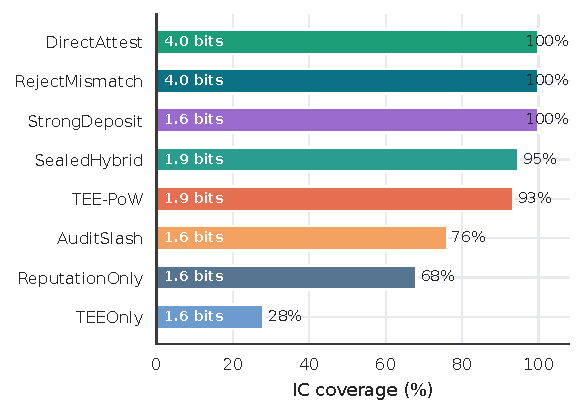
\includegraphics[width=0.84\columnwidth]{figures/disclosure_frontier.pdf}
\caption{Exact disclosure removes hidden premiums; sealed-class mechanisms trade budget confidentiality against residual deterrence.}
\label{fig:disclosure-frontier}
\end{figure}

\subsection{Valuation and Budget Fraud}

Fig.~\ref{fig:value-curves} shows representative $n=10^5$ valuation curves. Value rises with the realized LDP budget for all workloads. BRR is already high value at small $\eps_h$, while OUE and OLH need larger budgets to become commercially useful because their estimator variance is larger for medium and large domains. This monotonicity creates the economic attack surface: a seller can claim a large $\eps_c$ while using a stricter $\eps_h$ and still submit a formally private report.

\begin{figure}[t]
\centering
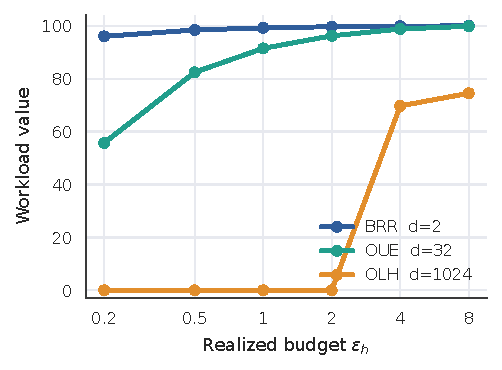
\includegraphics[width=0.84\columnwidth]{figures/valuation_curves.pdf}
\caption{Workload value rises with realized LDP budget for BRR, OUE, and OLH.}
\label{fig:value-curves}
\end{figure}

Fig.~\ref{fig:fraud-premium} quantifies the premium for OUE at $n=10^5,d_x=32$. The largest displayed premium is $44.1$ value units for $(\eps_h,\eps_c)=(0.2,8)$, and every valid over-claim cell has positive premium. Across the full sweep, the largest premium is $99.49$ value units for OUE with $n=10^4,d_x=32,(\eps_h,\eps_c)=(0.2,8)$. Table~\ref{tab:largest-premiums} lists the highest-premium regimes, which are the regimes where residual controls must be strongest.

\begin{figure}[t]
\centering
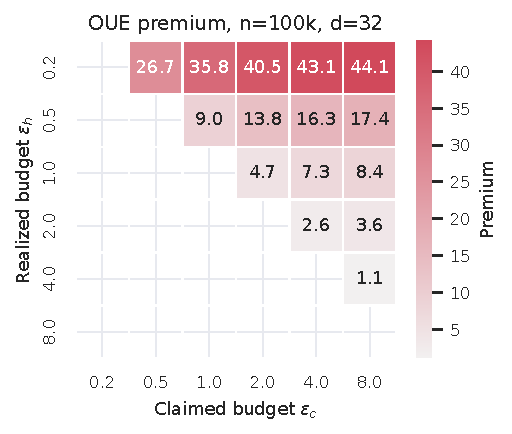
\includegraphics[width=0.84\columnwidth]{figures/fraud_premium_heatmap.pdf}
\caption{Over-claiming creates a positive OUE valuation premium for every $\eps_c>\eps_h$ cell.}
\label{fig:fraud-premium}
\end{figure}

\begin{table}[t]
\caption{Largest fraud-premium regimes in the valuation sweep.}
\label{tab:largest-premiums}
\centering
\scriptsize
\begin{tabular}{rrrrr}
\toprule
$n$ & $d_x$ & $\eps_h$ & $\eps_c$ & premium \\
\midrule
$10^4$ & 32 & 0.2 & 8 & 99.49 \\
$10^5$ & 1024 & 0.5 & 8 & 99.07 \\
$10^5$ & 1024 & 0.2 & 8 & 99.07 \\
$10^4$ & 1024 & 1 & 8 & 97.05 \\
$10^4$ & 1024 & 0.2 & 8 & 97.05 \\
\bottomrule
\end{tabular}
\end{table}

\subsection{Advertising-Style Marketing Workload}

Synthetic frequency curves alone do not capture the sparsity and long-tail structure of data marketing. We therefore evaluate a Criteo-style advertising telemetry schema with fields for user, campaign, segment, impression, click, and conversion. The workload contains 16 campaigns, 96 segments, 50k users, 525,916 impressions, 15,614 clicks, and 270 conversions. It supports three products that are commonly sold or measured in marketing pipelines: audience counts, segment reach, and conversion-rate sketches.

Fig.~\ref{fig:marketing-workload} summarizes the results. Audience counting is comparatively robust: mean relative error falls from $0.193$ at $\eps_h=0.5$ to $0.042$ at $\eps_h=2$ and $0.002$ at $\eps_h=8$. Segment reach is more sensitive, falling from $0.251$ to $0.054$ and $0.002$ over the same budgets. Conversion-rate sketches are the hardest product because conversions are sparse and top-segment allocation becomes unstable when long-tail segments are noisy. This workload is where a hidden budget gap creates the clearest business-decision regret.

\begin{figure*}[t]
\centering
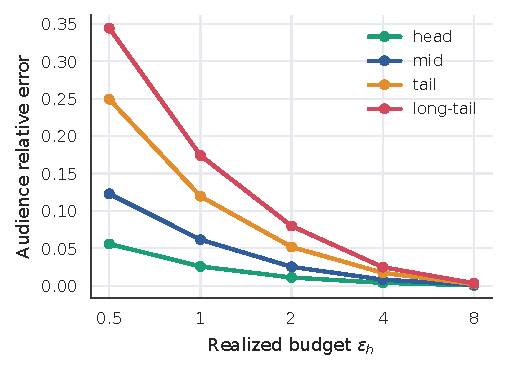
\includegraphics[width=0.28\textwidth]{figures/marketing_audience_error.pdf}\hfill
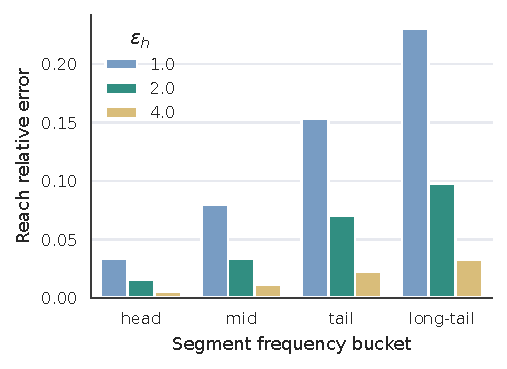
\includegraphics[width=0.28\textwidth]{figures/marketing_reach_error.pdf}\hfill
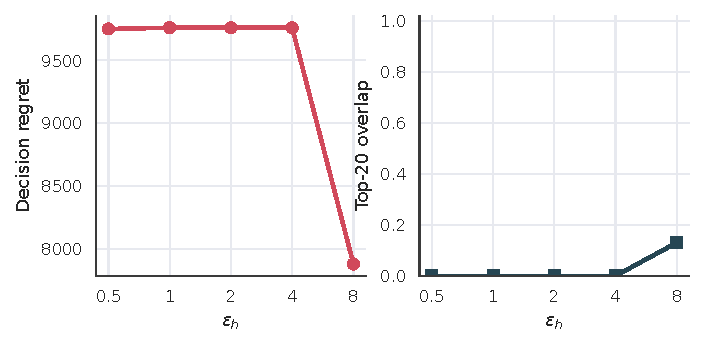
\includegraphics[width=0.28\textwidth]{figures/marketing_conversion_regret.pdf}
\caption{The advertising-style workload shows that audience counting is easier than long-tail reach and sparse conversion-rate decisions.}
\label{fig:marketing-workload}
\end{figure*}

Fig.~\ref{fig:marketing-frontier} applies the disclosure-regime analysis to the marketing workload. Exact disclosure again eliminates hidden premiums. Sealed-class mechanisms preserve budget confidentiality and require residual deterrence; among those, \Hybrid{} is the strongest option when full escrow is unavailable.

\begin{figure}[t]
\centering
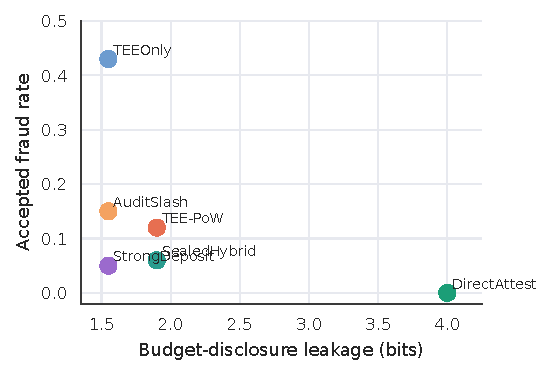
\includegraphics[width=0.72\columnwidth]{figures/marketing_disclosure_frontier.pdf}
\caption{The marketing workload separates exact-disclosure and sealed-class deterrence regimes.}
\label{fig:marketing-frontier}
\end{figure}

\subsection{AWS Nitro TEE Evidence}

The hardware experiment runs the LDP oracle inside AWS Nitro Enclaves. The non-debug pilot run stores 50 NSM attestation COSE documents, response JSON files, raw latency rows, EIF hashes, PCR prefixes, parent diagnostics, and a result manifest. Table~\ref{tab:aws} summarizes the run. The mean enclave oracle time is $2.21$ ms and the mean attestation-generation time is $2.10$ ms. The client-side PoW solve at $k=15$ dominates the pilot path, with mean $32.74$ ms and p95 $70.75$ ms; the TEE and attestation path are small relative to that optional residual cost.

\begin{table}[t]
\caption{AWS Nitro Enclaves pilot uses the real NSM attestation path.}
\label{tab:aws}
\centering
\footnotesize
\begin{tabularx}{\columnwidth}{p{0.34\columnwidth}X}
\toprule
Item & Measurement \\
\midrule
Run & \texttt{icde-ldp-nitro-20260605094208} \\
Parent host & \texttt{m6i.xlarge}, \texttt{us-east-2a}, Amazon Linux 2023.11 \\
Enclave allocation & 2 vCPUs, 2048 MiB, CID 16, non-debug launch \\
Image identity & EIF prefix \texttt{0f97a460}; PCR prefixes \texttt{faa4049a}, \texttt{4b4d5b36}, \texttt{5e84099a} \\
Reports & 50 LDP reports and 50 Nitro NSM documents \\
Oracle latency & mean 2.21 ms; p95 2.33 ms \\
Attestation & mean 2.10 ms; p95 2.22 ms \\
Vsock round trip & mean 3.37 ms; p95 3.71 ms \\
PoW solve & $k=15$; mean 32.74 ms; p95 70.75 ms \\
\bottomrule
\end{tabularx}
\end{table}

The replay and downgrade tests in Fig.~\ref{fig:nitro-replay} mutate response metadata from the Nitro run. The full verifier accepts only fresh reports with expected PCRs, a verifier nonce, a monotone counter, a bound report commitment, and a matching residual-control target. Removing a check exposes exactly the failure that check is meant to prevent: stale counters pass only without counter checking, mismatched PCRs pass only without PCR checking, and modified difficulty buckets pass only without PoW binding.

\begin{figure*}[t]
\centering
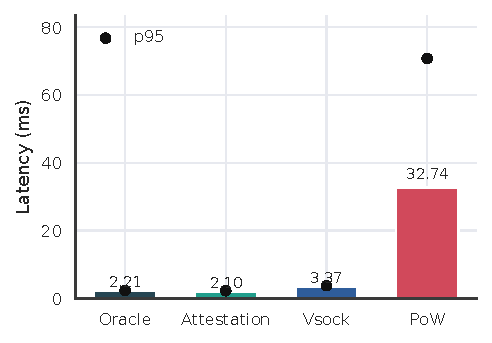
\includegraphics[width=0.38\textwidth]{figures/nitro_latency.pdf}
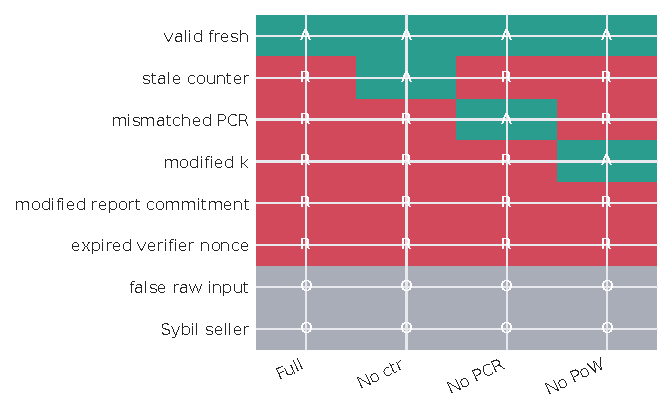
\includegraphics[width=0.38\textwidth]{figures/replay_confusion.pdf}
\caption{Nitro latency is small relative to optional PoW, and full verification rejects replay and downgrade mutations.}
\label{fig:nitro-replay}
\end{figure*}

\subsection{Optional PoW Calibration}

Because PoW is not the default residual control, the calibration experiment is a stress test for the settings where a platform wants rate limiting or cannot use monetary escrow. The Nitro-calibrated effective hash rate implied by the $k=15$ pilot is $1.00\times 10^6$ hashes/s, while the local Python microbenchmark is about $3.4\times 10^6$ hashes/s. Fig.~\ref{fig:pow} shows exponential growth in mean and p95 solve time. The honest baseline region $k\in[14,16]$ stays below $100$ ms p95 in observed local solves; larger buckets quickly become deadline-heavy and are better handled by deposits or rejection.

\begin{figure*}[t]
\centering
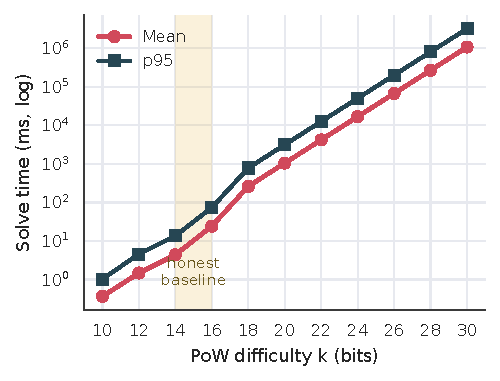
\includegraphics[width=0.38\textwidth]{figures/pow_calibration.pdf}
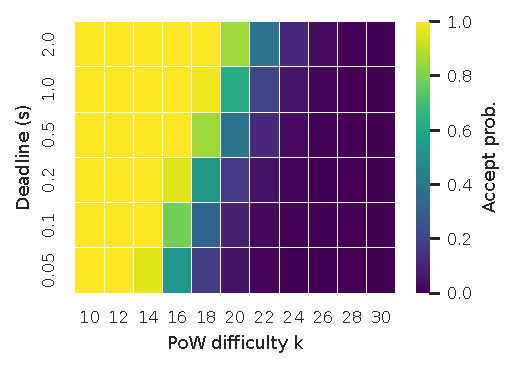
\includegraphics[width=0.38\textwidth]{figures/pow_deadline_heatmap.pdf}
\caption{Optional PoW solve time grows exponentially with $k$, and deadline admission separates honest and high-premium buckets.}
\label{fig:pow}
\end{figure*}

\begin{table}[t]
\caption{PoW calibration maps premium buckets to operational actions.}
\label{tab:pow}
\centering
\scriptsize
\begin{tabularx}{\columnwidth}{rrrrX}
\toprule
$k$ & trials & mean ms & p95 ms & use \\
\midrule
14 & 32 & 4.4 & 13.5 & low-latency honest baseline \\
16 & 16 & 24.2 & 73.1 & high-SLA honest or small gap \\
20 & model & 1047.83 & 3139.01 & small-to-medium premium \\
24 & model & 16765.22 & 50224.11 & large premium with relaxed deadline \\
28 & model & 268243.54 & 803585.84 & deposit or reject \\
\bottomrule
\end{tabularx}
\end{table}

\subsection{Incentives and Market Utility}

The payoff sweep combines the valuation premiums with each mechanism's residual cost. Fig.~\ref{fig:ic} reports the best coverage achieved by each mechanism and the hybrid sensitivity grid. \NoVerify{} covers only $9.3\%$ of over-claim cells. \DirectAttest{} and \RejectMismatch{} cover all cells by exact disclosure. In sealed-class disclosure, \TEEOnly{} covers $26.7\%$, \AuditSlash{} covers $74.7\%$, \ReputationOnly{} covers $68.0\%$, \TEEPOW{} reaches $93.3\%$ at $\lambda=2$, and \Hybrid{} reaches $94.7\%$ when deposits absorb the largest premium buckets. The cells that remain non-IC are informative: their premiums are too large for a practical latency budget, so the market should require escrow or reject the class mismatch.

\begin{figure*}[t]
\centering
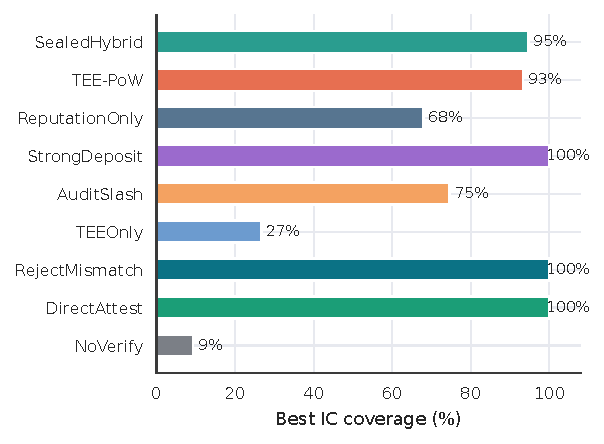
\includegraphics[width=0.38\textwidth]{figures/ic_coverage.pdf}
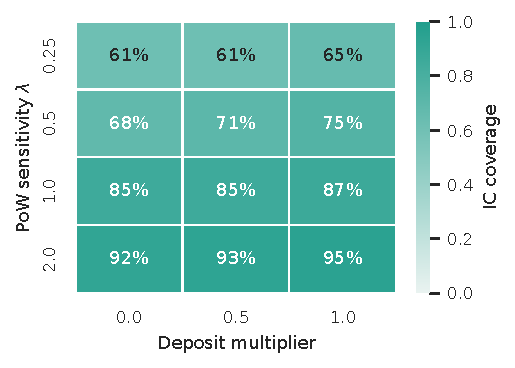
\includegraphics[width=0.38\textwidth]{figures/ic_coverage_heatmap.pdf}
\caption{Gap-indexed residual controls expand the incentive-compatible region.}
\label{fig:ic}
\end{figure*}

The end-to-end marketing simulation includes buyers, honest sellers, fraudulent sellers, LDP aggregation, market acceptance, and downstream campaign allocation scored against the advertising-workload ground truth. Fig.~\ref{fig:market-utility} reports averages over seeds $\{2026,\ldots,2030\}$. Because conversion-rate sketches are sparse, the no-fraud upper region is around 19 buyer-utility units. At fraudulent-seller fraction $\rho=0.7$, \NoVerify{} buyer utility falls to $0.62$ and accepted fraud reaches $0.644$. \DirectAttest{} keeps accepted fraud at zero and buyer utility at $18.62$ when exact disclosure is allowed. Among sealed-class designs, \StrongDeposit{} reaches buyer utility $17.00$ with accepted fraud $0.042$, while \Hybrid{} keeps accepted fraud to $0.049$ and buyer utility to $14.76$ without requiring full escrow.

\begin{figure*}[t]
\centering
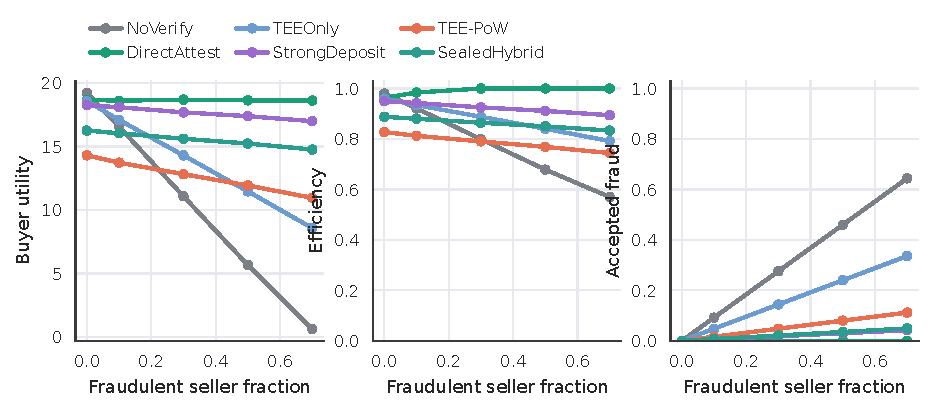
\includegraphics[width=0.76\textwidth]{figures/market_utility.pdf}
\caption{Buyer utility and efficiency recover when accepted fraudulent reports are suppressed.}
\label{fig:market-utility}
\vspace{-3mm}
\end{figure*}

Fig.~\ref{fig:market-baselines} fixes $\rho=0.7$. \NoVerify{} accepts $0.644$ fraudulent reports on average and buyer utility falls to $1.74$. \DirectAttest{} and \RejectMismatch{} keep accepted fraud at zero; \StrongDeposit{} and \Hybrid{} reduce accepted fraud to $0.042$ and $0.049$, respectively.

\begin{figure}[t]
\centering
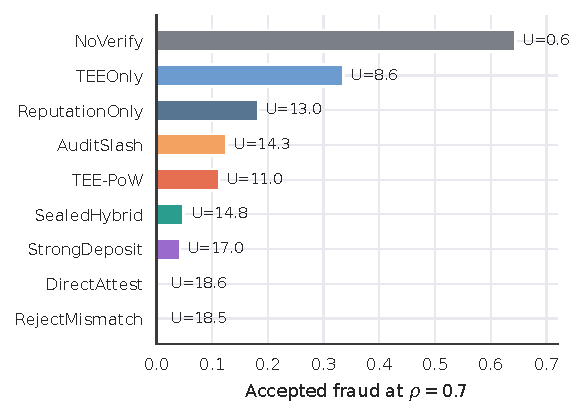
\includegraphics[width=0.72\columnwidth]{figures/market_baselines.pdf}
\caption{At $\rho=0.7$, exact-disclosure and escrow baselines provide the lowest accepted fraud.}
\label{fig:market-baselines}
\vspace{-3mm}
\end{figure}

\subsection{Robustness and Scalability}

Fig.~\ref{fig:robustness} stresses deployment choices. Narrow difficulty buckets improve IC coverage but increase p95 latency and reveal more budget-class information. Hash-rate heterogeneity raises tail latency and reduces IC coverage because stronger sellers can solve expensive buckets more easily. Deposit share $0.5$ gives $94\%$ IC coverage with p95 latency $62$ ms; all-deposit policies reduce latency but lose some deterrence when deposits are capped by contract.

\begin{figure}[t]
\centering
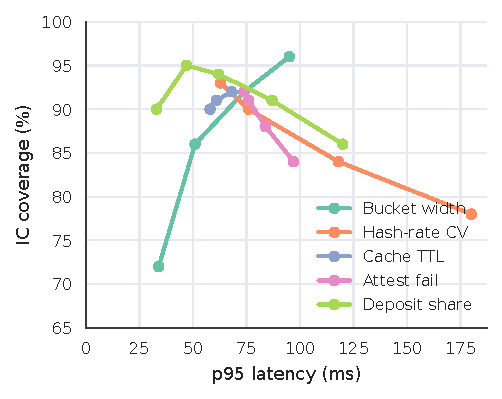
\includegraphics[width=0.72\columnwidth]{figures/robustness_ablation.pdf}
\caption{Robustness ablations expose latency, leakage, and incentive-coverage trade-offs.}
\label{fig:robustness}
\vspace{-3mm}
\end{figure}

The scaled Nitro run uses an \texttt{m6i.xlarge} parent in \texttt{us-east-2a}, a 2-vCPU/2048 MiB enclave, batch size 128, and an EC2 parent price assumption of $\$0.192$/h. \mbox{Fig.~\ref{fig:throughput-cost} and Table~\ref{tab:throughput-cost}} report measured throughput and cost for the standard phases. \DirectAttest{} and \TEEOnly{} each process one million reports at about $666.6$ reports/s with p95 latency about $18.9$ ms. Optional PoW is the bottleneck: \TEEPOW{} at $k=15$ processes 250k reports at $29.4$ reports/s, while \Hybrid{} at $k=14$ processes 500k reports at $57.5$ reports/s. The result supports the design choice: high-throughput markets should rely on direct attestation, rejection, deposits, and audits first, using PoW only for throttling or escrow-constrained contracts.

The scale run produced 2.76 million measured reports over 5.86 hours. The EIF hash prefix is \texttt{f1d9dde8}; PCR0/PCR1/PCR2 prefixes are \texttt{c189c18e}, \texttt{4b4d5b36}, and \texttt{fe3b5422}. All primary throughput rows in Table~\ref{tab:throughput-cost} are measured on the Nitro path. The run stores every per-report latency row, all attestation documents for the 10k correctness phase, and a sampled attestation set for scale phases, yielding 10,335 COSE documents and matching response files.

\begin{figure}[t]
\centering
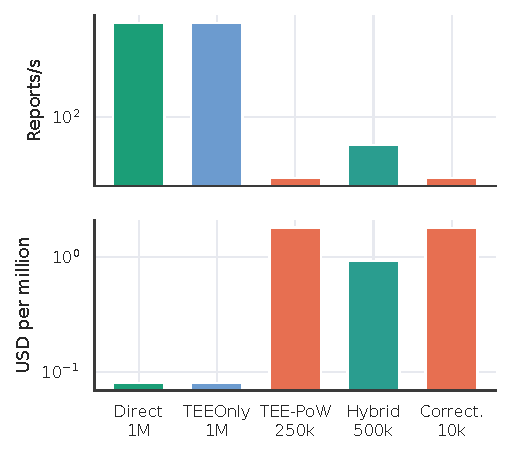
\includegraphics[width=0.72\columnwidth]{figures/throughput_cost.pdf}
\caption{Scaled Nitro phases show exact-attestation baselines and optional-PoW bottlenecks.}
\label{fig:throughput-cost}
\end{figure}

\begin{table}[!b]
\caption{Scaled AWS Nitro measurements provide throughput and cost.}
\label{tab:throughput-cost}
\centering
\scriptsize
\begin{tabular}{lrrrr}
\toprule
Phase & reports & reports/s & p95 ms & USD/M \\
\midrule
\DirectAttest{} & 1,000,000 & 666.6 & 18.9 & 0.080 \\
\TEEOnly{} & 1,000,000 & 666.7 & 18.9 & 0.080 \\
\TEEPOW{} ($k=15$) & 250,000 & 29.4 & 643.4 & 1.813 \\
\Hybrid{} ($k=14$) & 500,000 & 57.5 & 305.2 & 0.928 \\
Correctness ($k=15$) & 10,000 & 29.5 & 264.9 & 1.810 \\
\bottomrule
\end{tabular}
\end{table}

\subsection{Adaptive Attackers and Verification Controls}

The adaptive-attacker simulation lets sellers choose among truthful submission, fixed over-claiming, adaptive over-claiming, and replay/downgrade attempts. Fig.~\ref{fig:attacker} shows accepted fraud as a function of residual-control sensitivity. \NoVerify{} remains vulnerable with accepted fraud $0.88$ at $\lambda=1$, and \TEEOnly{} remains vulnerable to class-boundary gaming at $0.56$. Exact-disclosure baselines reject the over-claiming strategy. \StrongDeposit{} and \Hybrid{} switch to truthful behavior under moderate sensitivity and deposits; at $\lambda=1$ and deposit multiplier $1$, both keep accepted fraud at $0.03$ over $10^4$ simulated rounds per cell.

\begin{figure}[t]
\centering
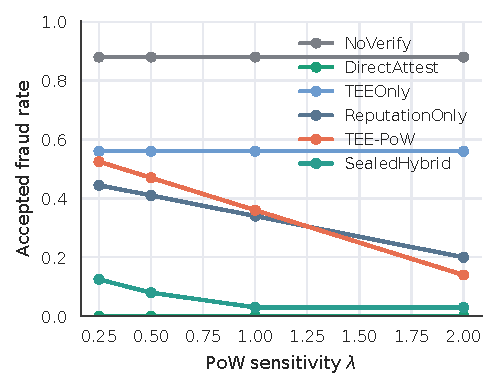
\includegraphics[width=0.72\columnwidth]{figures/attacker_strategy.pdf}
\caption{Adaptive sellers switch to truthful behavior when hybrid deterrence dominates the premium.}
\label{fig:attacker}
\end{figure}

Table~\ref{tab:negative-controls} reports the negative-control matrix used to audit the verifier. Each disabled-check column admits exactly the mutation that check is meant to catch, while the full verifier rejects stale counters, mismatched PCRs, modified difficulty targets, modified report commitments, and expired verifier nonces. False raw inputs and Sybil sellers are handled by the upstream provenance and identity layer identified in Table~\ref{tab:threat-boundary}.

\begin{table}[t]
\caption{Negative controls identify which verifier check is necessary.}
\label{tab:negative-controls}
\centering
\scriptsize
\begin{tabularx}{\columnwidth}{p{0.32\columnwidth}X}
\toprule
Control & Observed failure when disabled \\
\midrule
No counter check & stale counter is accepted \\
No PCR allow-list & mismatched enclave measurement is accepted \\
No PoW binding & modified difficulty target is accepted \\
No report commitment & modified report is not bound to attestation \\
\TEEOnly{} & class-boundary over-claim remains profitable \\
Single coarse bucket & high-premium fraud is underpriced \\
\bottomrule
\end{tabularx}
\end{table}

\subsection{Reproducibility}

Each plotted value is backed by a typed result file, and each figure is regenerated from the same tables used by the paper. Hardware results are tied to the recorded Nitro manifests, EIF hashes, PCR prefixes, and run identifiers above. This makes the synthetic valuation sweeps, marketing workload, incentive sweeps, and scaled Nitro measurements independently auditable without presenting mock TEE latency as hardware evidence.

\section{Conclusion}

LDP data products need verifiable execution identity in addition to a formal privacy definition. This paper introduced budget-integrity certificates for LDP data markets, showed how exact-disclosure baselines and sealed-class contracts lead to different mechanisms, and instantiated the sealed-class case with a TEE-sealed local oracle. The empirical results show that exact attestation is the simplest option when exact $\eps_h$ may be public, while sealed-class markets can combine attestation with deposits, audits, reputation, and optional PoW to deter hidden budget over-claims. The Nitro measurements indicate that the TEE and attestation path is practical, and that PoW should remain a selective residual signal rather than the default path for high-throughput markets.

\section*{AI-Generated Content Acknowledgment}
Generative AI tools, including OpenAI ChatGPT/Codex-style assistants, were used for language editing and implementation support such as code-formatting assistance. No AI system is listed as an author. The authors reviewed and manually verified all technical claims, proofs, code, experimental results, figures, and final text.

\begin{thebibliography}{99}
\bibitem{duchi2013local}
J. C. Duchi, M. I. Jordan, and M. J. Wainwright, ``Local privacy and statistical minimax rates,'' in \emph{IEEE FOCS}, 2013, pp. 429--438.

\bibitem{kasiviswanathan2011what}
S. P. Kasiviswanathan, H. K. Lee, K. Nissim, S. Raskhodnikova, and A. Smith, ``What can we learn privately?'' \emph{SIAM Journal on Computing}, vol. 40, no. 3, pp. 793--826, 2011.

\bibitem{erlingsson2014rappor}
U. Erlingsson, V. Pihur, and A. Korolova, ``Rappor: Randomized aggregatable privacy-preserving ordinal response,'' in \emph{ACM CCS}, 2014, pp. 1054--1067.

\bibitem{Wang2017LDPFreq}
T. Wang, J. Blocki, N. Li, and S. Jha, ``Locally differentially private protocols for frequency estimation,'' in \emph{USENIX Security}, 2017, pp. 729--745.

\bibitem{koutris2012query}
P. Koutris, P. Upadhyaya, M. Balazinska, B. Howe, and D. Suciu, ``Query-based data pricing,'' in \emph{PODS}, 2012, pp. 167--178.

\bibitem{li2014pricing}
C. Li, D. Y. Li, G. Miklau, and D. Suciu, ``A theory of pricing private data,'' in \emph{ICDT}, 2014, pp. 33--44.

\bibitem{deep2017design}
S. Deep and P. Koutris, ``The design of arbitrage-free data pricing schemes,'' in \emph{ICDT}, LIPIcs, vol. 68, 2017, pp. 12:1--12:18.

\bibitem{qirana2017}
S. Deep and P. Koutris, ``QIRANA: A framework for scalable query pricing,'' in \emph{ACM SIGMOD}, 2017, pp. 699--713.

\bibitem{ghosh2011selling}
A. Ghosh and A. Roth, ``Selling privacy at auction,'' in \emph{ACM EC}, 2011, pp. 199--208.

\bibitem{agarwal2019marketplace}
A. Agarwal, M. Dahleh, and T. Sarkar, ``A marketplace for data: An algorithmic solution,'' in \emph{ACM EC}, 2019, pp. 701--726.

\bibitem{chen2022privacy}
X. Chen, D. Simchi-Levi, and Y. Wang, ``Privacy-preserving dynamic personalized pricing with demand learning,'' \emph{Management Science}, vol. 68, no. 7, pp. 4878--4898, 2022.

\bibitem{chen2023privacy}
X. Chen, S. Miao, and Y. Wang, ``Differential privacy in personalized pricing with nonparametric demand models,'' \emph{Operations Research}, vol. 71, no. 2, pp. 581--602, 2023.

\bibitem{lei2024privacy}
Y. Lei, S. Miao, and R. Momot, ``Privacy-preserving personalized revenue management,'' \emph{Management Science}, vol. 70, no. 7, pp. 4875--4892, 2024.

\bibitem{cheu2021manipulation}
A. Cheu, A. Smith, and J. Ullman, ``Manipulation attacks in local differential privacy,'' in \emph{IEEE Symposium on Security and Privacy}, 2021, pp. 883--900.

\bibitem{cao2021data}
X. Cao, J. Jia, and N. Z. Gong, ``Data poisoning attacks to local differential privacy protocols,'' in \emph{USENIX Security}, 2021, pp. 947--964.

\bibitem{wu2021poisoning}
Y. Wu, X. Cao, J. Jia, and N. Z. Gong, ``Poisoning attacks to local differential privacy protocols for key-value data,'' in \emph{USENIX Security}, 2022, pp. 519--536.

\bibitem{kato2021verifiable}
F. Kato, Y. Cao, and M. Yoshikawa, ``Preventing manipulation attack in local differential privacy using verifiable randomization mechanism,'' in \emph{DBSec}, 2021, pp. 43--60.

\bibitem{rogers2016odometers}
R. M. Rogers, A. Roth, J. Ullman, and S. Vadhan, ``Privacy odometers and filters: Pay-as-you-go composition,'' in \emph{NeurIPS}, 2016, pp. 1921--1929.

\bibitem{spence1973job}
M. Spence, ``Job market signaling,'' \emph{Quarterly Journal of Economics}, vol. 87, no. 3, pp. 355--374, 1973.

\bibitem{back2002hashcash}
A. Back, ``Hashcash - a denial of service counter-measure,'' Tech. Rep., 2002.

\bibitem{nakamoto2008bitcoin}
S. Nakamoto, ``Bitcoin: A peer-to-peer electronic cash system,'' 2008. [Online]. Available: \url{https://bitcoin.org/bitcoin.pdf}

\bibitem{kroll2013economics}
J. A. Kroll, I. C. Davey, and E. W. Felten, ``The economics of Bitcoin mining, or Bitcoin in the presence of adversaries,'' in \emph{WEIS}, 2013.

\bibitem{eyal2014majority}
I. Eyal and E. G. Sirer, ``Majority is not enough: Bitcoin mining is vulnerable,'' in \emph{Financial Cryptography}, LNCS, vol. 8437, 2014, pp. 436--454.

\bibitem{costan2016intel}
V. Costan and S. Devadas, ``Intel SGX explained,'' IACR Cryptology ePrint Archive, Report 2016/086, 2016.

\bibitem{awsnitro}
Amazon Web Services, ``AWS Nitro Enclaves User Guide,'' \url{https://docs.aws.amazon.com/enclaves/latest/user/nitro-enclave.html}, accessed Jun. 5, 2026.

\bibitem{awsattest}
Amazon Web Services, ``Cryptographic attestation in AWS Nitro Enclaves,'' \url{https://docs.aws.amazon.com/enclaves/latest/user/set-up-attestation.html}, accessed Jun. 5, 2026.

\bibitem{buneman2001provenance}
P. Buneman, S. Khanna, and W.-C. Tan, ``Why and where: A characterization of data provenance,'' in \emph{ICDT}, 2001, pp. 316--330.

\bibitem{green2007provenance}
T. J. Green, G. Karvounarakis, and V. Tannen, ``Provenance semirings,'' in \emph{PODS}, 2007, pp. 31--40.

\bibitem{schuster2015vc3}
F. Schuster, M. Costa, C. Fournet, C. Gkantsidis, M. Peinado, G. Mainar-Ruiz, and M. Russinovich, ``VC3: Trustworthy data analytics in the cloud using SGX,'' in \emph{IEEE Symposium on Security and Privacy}, 2015, pp. 38--54.

\bibitem{zheng2017opaque}
W. Zheng, A. Dave, J. G. Beekman, R. A. Popa, J. E. Gonzalez, and I. Stoica, ``Opaque: An oblivious and encrypted distributed analytics platform,'' in \emph{NSDI}, 2017, pp. 283--298.

\bibitem{priebe2018enclavedb}
C. Priebe, D. Muthukumaran, D. O'Keeffe, D. Eyers, B. Shand, and P. Pietzuch, ``EnclaveDB: A secure database using SGX,'' in \emph{IEEE Symposium on Security and Privacy}, 2018, pp. 264--278.

\end{thebibliography}

\end{document}
